\section{Validation} \label{s:N_II:validation}


This part of the chapter contains different comparisons and network metrics analyses to test and validate the changes made to the network pipeline. The graph changes between a tumour and non-tumour network are presented in \cref{s:N_II:net_comp}, the difference in the two reward functions are presented in \cref{s:N_II:reward_comp} and the effects of the integrative MEV introduced to the MIBC subtypes are covered in \cref{s:N_II:mev_comp}. The difference in the community detection algorithms is not covered as the \acrfull{hsbm} is just a nested SBM which allows to discover more communities than the standard SBM; the comparison between Leiden and SBM was covered in \cref{s:gene_sel}.


% Network validation 
\subsection{Non-tumour vs Tumour Network} \label{s:N_II:net_comp}

To study the differences between the non-tumour and tumour networks the previously used graph metrics (degree, pageRank, closeness, betwenees and IVI)\footnote{Reminder: the degree - node's number of connections; pageRank - node's centrality; closeness - how close the nodes are; betwenees - nodes between; IVI - a combination of network metrics} are shown in \cref{fig:N_II:net_metrics_comp}. There are four networks compared, the standard (red) and reward (green) for tumour derived, and the correspondent for non-tumour (mustard - standard and blue - reward).

% Degreee & PageRank
In the pageRank and degree metrics, the non-tumour networks seems to be elongated on the Y-axis, denoting a a high variance between the nodes. This is further enforced by the reward modifier, suggesting that there is a subset of nodes that have a high number of connections and are central to the network. Compared to the non-tumour, the TCGA derived graphs have nodes have similar values for centrality and degree. 

% Closeness & betweneess
A distinct feature of the tumour networks is that there the there is a subset of genes that are adjacent given by the closeness plot. The reward non-tumour network has the nodes closer compared with the standard, indicating the reward modifier 'brings' the node closer. Another distinct feature of the tumour networks is that these are characterised by a high value in betweeness, suggesting that there are several important nodes into the network.. Again, the reward modifier amplifies this compared to the standard.

% IVI
The IVI distribution for the two tumour networks are largely similar, but there is a noticeable difference between the non-tumour standard and reward graphs. It can be seen that the when the weight modifier is applied, the metric's distribution is sparser, havig a subset of genes that have higher values.

Overall the metrics comparisons shows that the non-tumour network react stronger to the sigmoid modifier and that there is a subset of genes that are more central and have a large number of connections; this is explored in more detail in \cref{s:N_II:high_conn}.

\begin{figure}[!htb]    
    \centering
    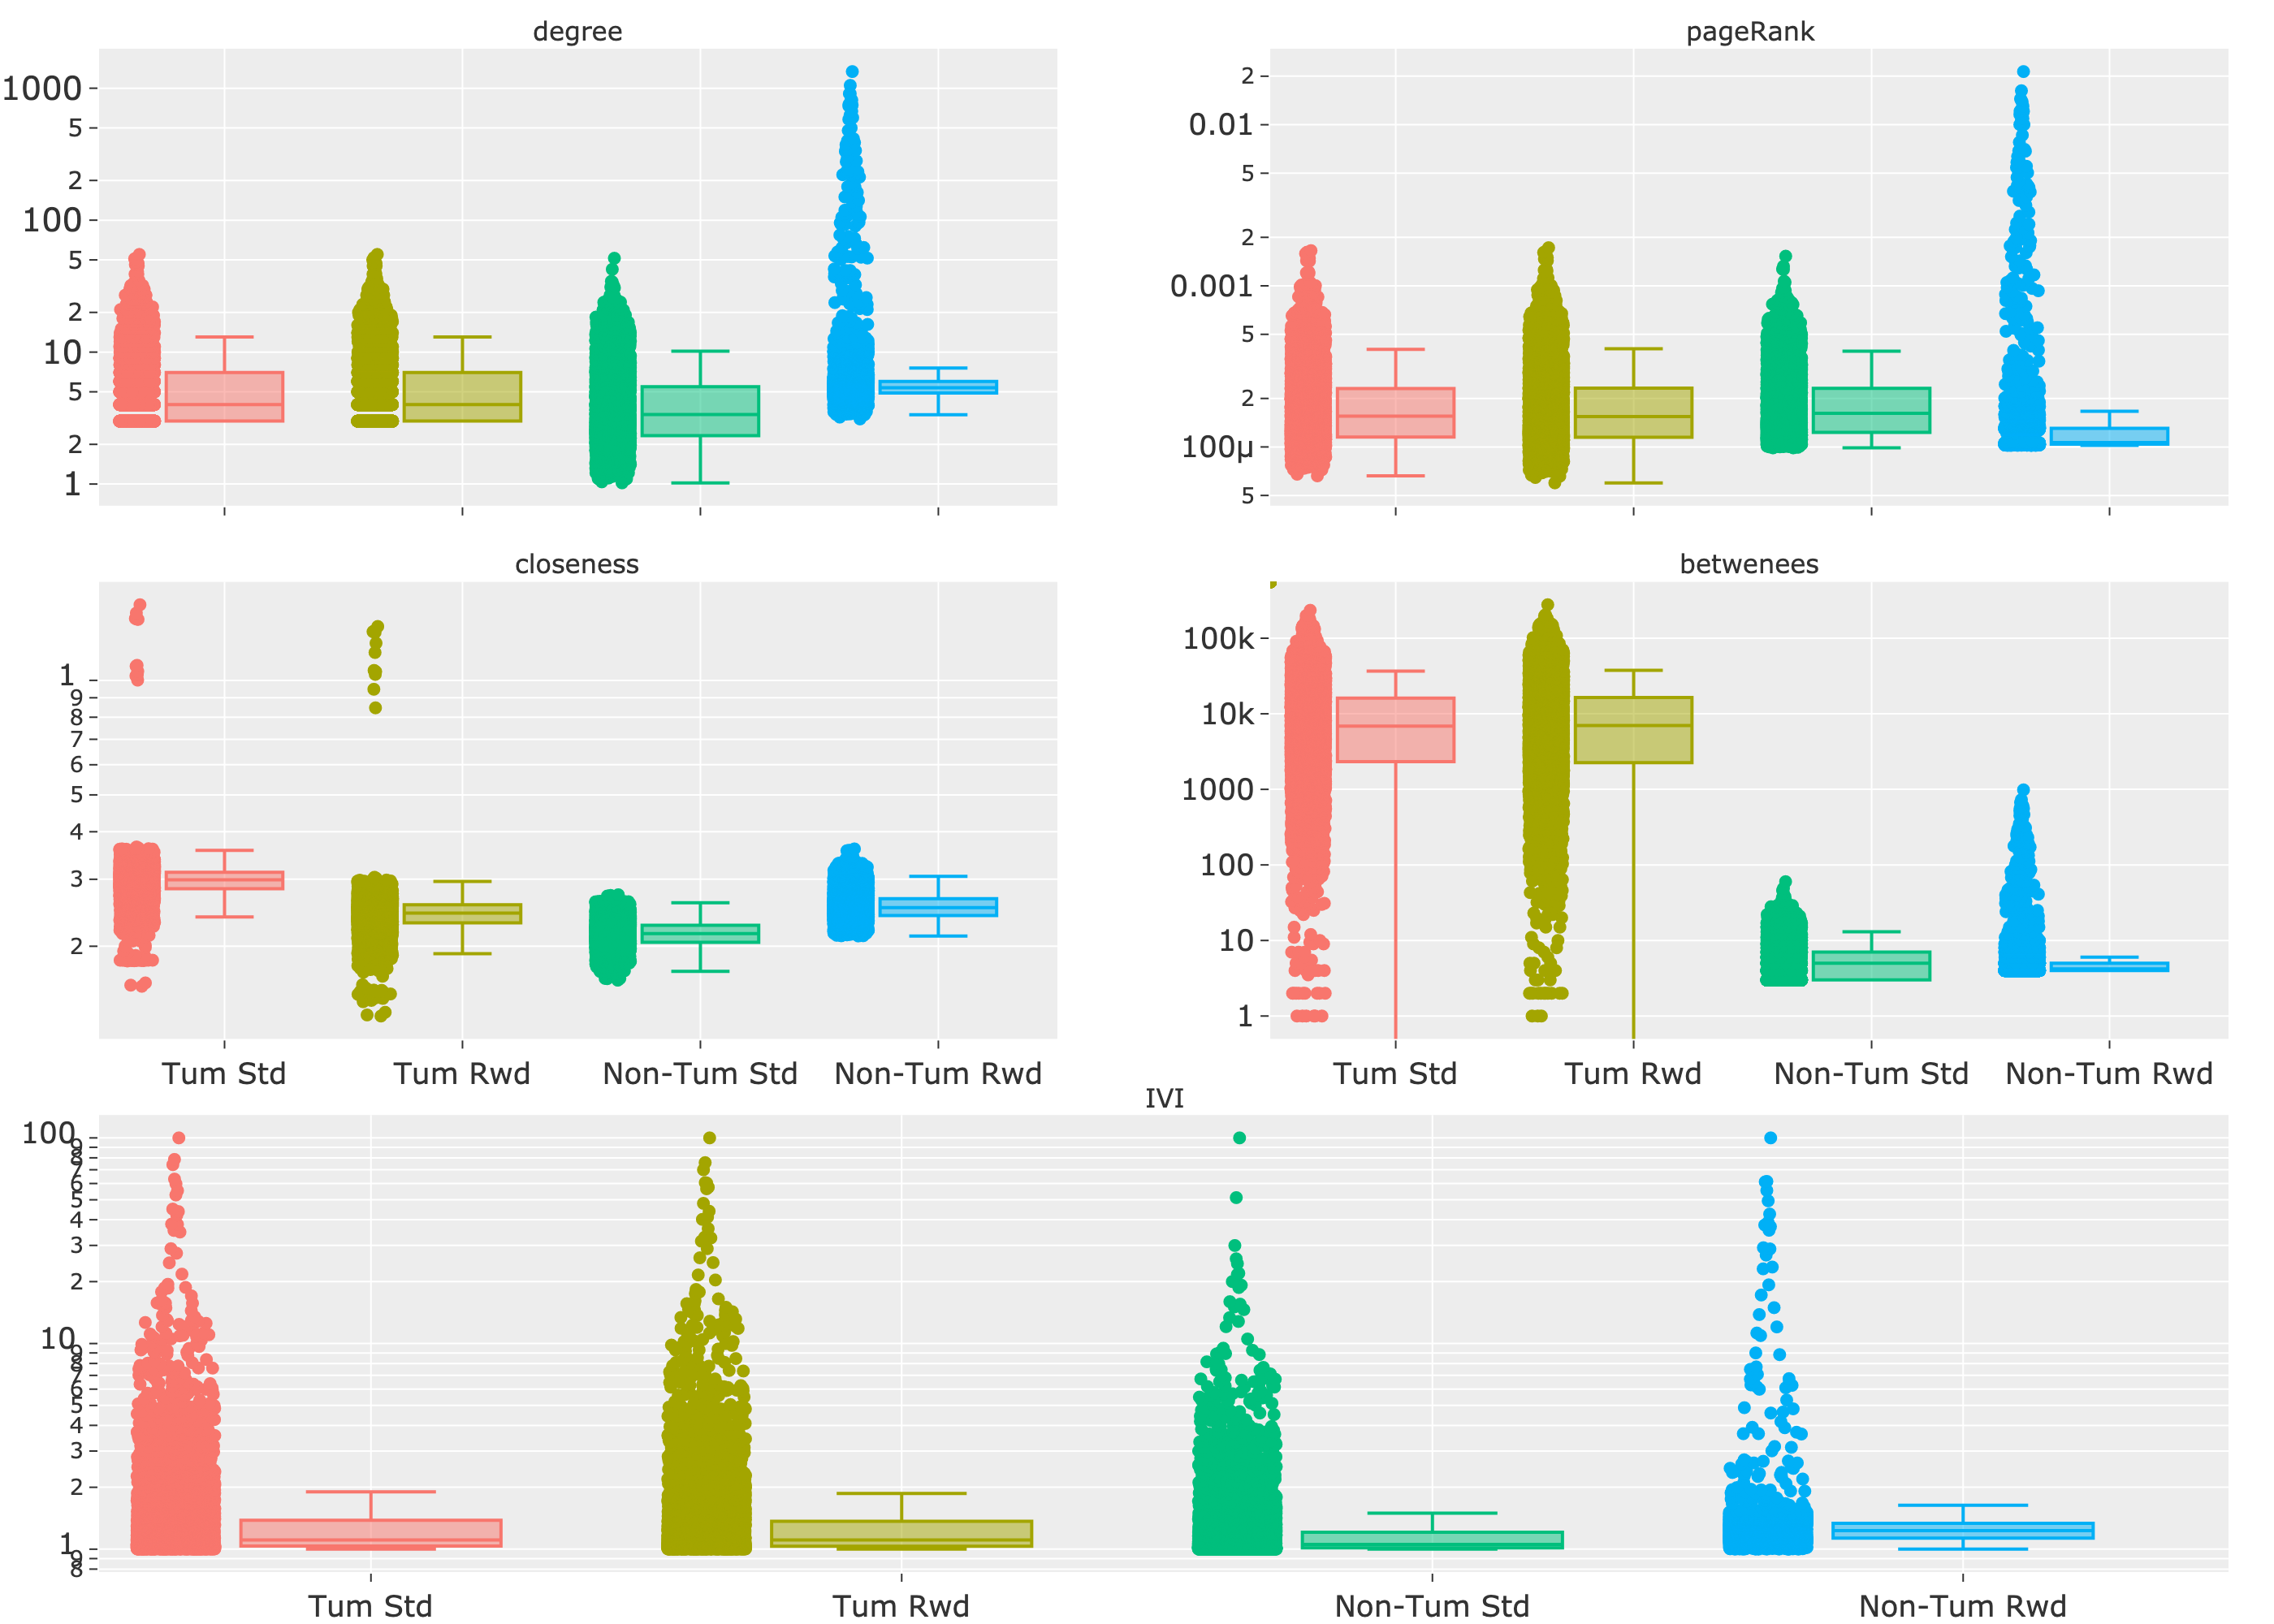
\includegraphics[width=1.0\textwidth,height=0.7\textheight,keepaspectratio]{Sections/Network_II/validation/network_comparison.png}
    \caption{Network metrics for the Tumour and non-tumour networks with no modifier and reward modifier. The y-axis represent the log10 of the metric.  See \cref{s:lit:netr_metrics} for a description of the metrics. }
    \label{fig:N_II:net_metrics_comp}
\end{figure}


% Reward 1 vs Reward v2
\subsection{Comparison between reward functions} \label{s:N_II:reward_comp}



% Do I need the following two paragraphs?
A sigmoid function is used as a reward modifier for the revised network pipeline presented in this chapter. The differences in how the weights are changed by the two functions is shown in \cref{s:N_II:reward}. The networks effects of the two reward functions on the network is studied in this section.

In the previous sections the network differences between the Standard and modified networks was studied through the bar plots. The comparisons involved three networks as 3 histograms on a single plot resulted on a cluttered figures. In this section, only the Standard and the Reward with sigmoid function are compared over the five usual clustering metrics utilised in this PhD project as well as the Katz Centrality metrics. The latter is a centrality metric available in the Graph-tool package\footnote{The Katz Centrality metric was available only in the Graph-tool package and not in the iGraph the package used by PGCNA to generated the graph.} which considers both the neighbours of a node as well as their connection over the network. Higher values means that the nodes are important both locally and globally in the network, while lower values are associated with less important roles. 

% Analyse the metrics
The six metric are shown in \cref{fig:N_II:net_metric_sig_std} where the x-axes represents the graph metric while the y-axes the log10 count, the orange is associated with the Reward and blue with the Standard network. Across all six plots there is a striking difference between the Standard and the Reward modifier,  in the latter graph the nodes' attributes are more spread compared to the unmodified network. This means that the nodes in the Standard graph have a relative similar importance, closeness into the network compared to the Reward which has a few number of genes that are highly connected, central to the network.
The distributions of the closeness metric suggests that the nodes in the modified graph are closer together compared to the un-modified one. The metrics suggests that the modifier have a large impact on to the network.


% Talk about the stats and the difference between the stats
\begin{figure}[H]    
    \centering
    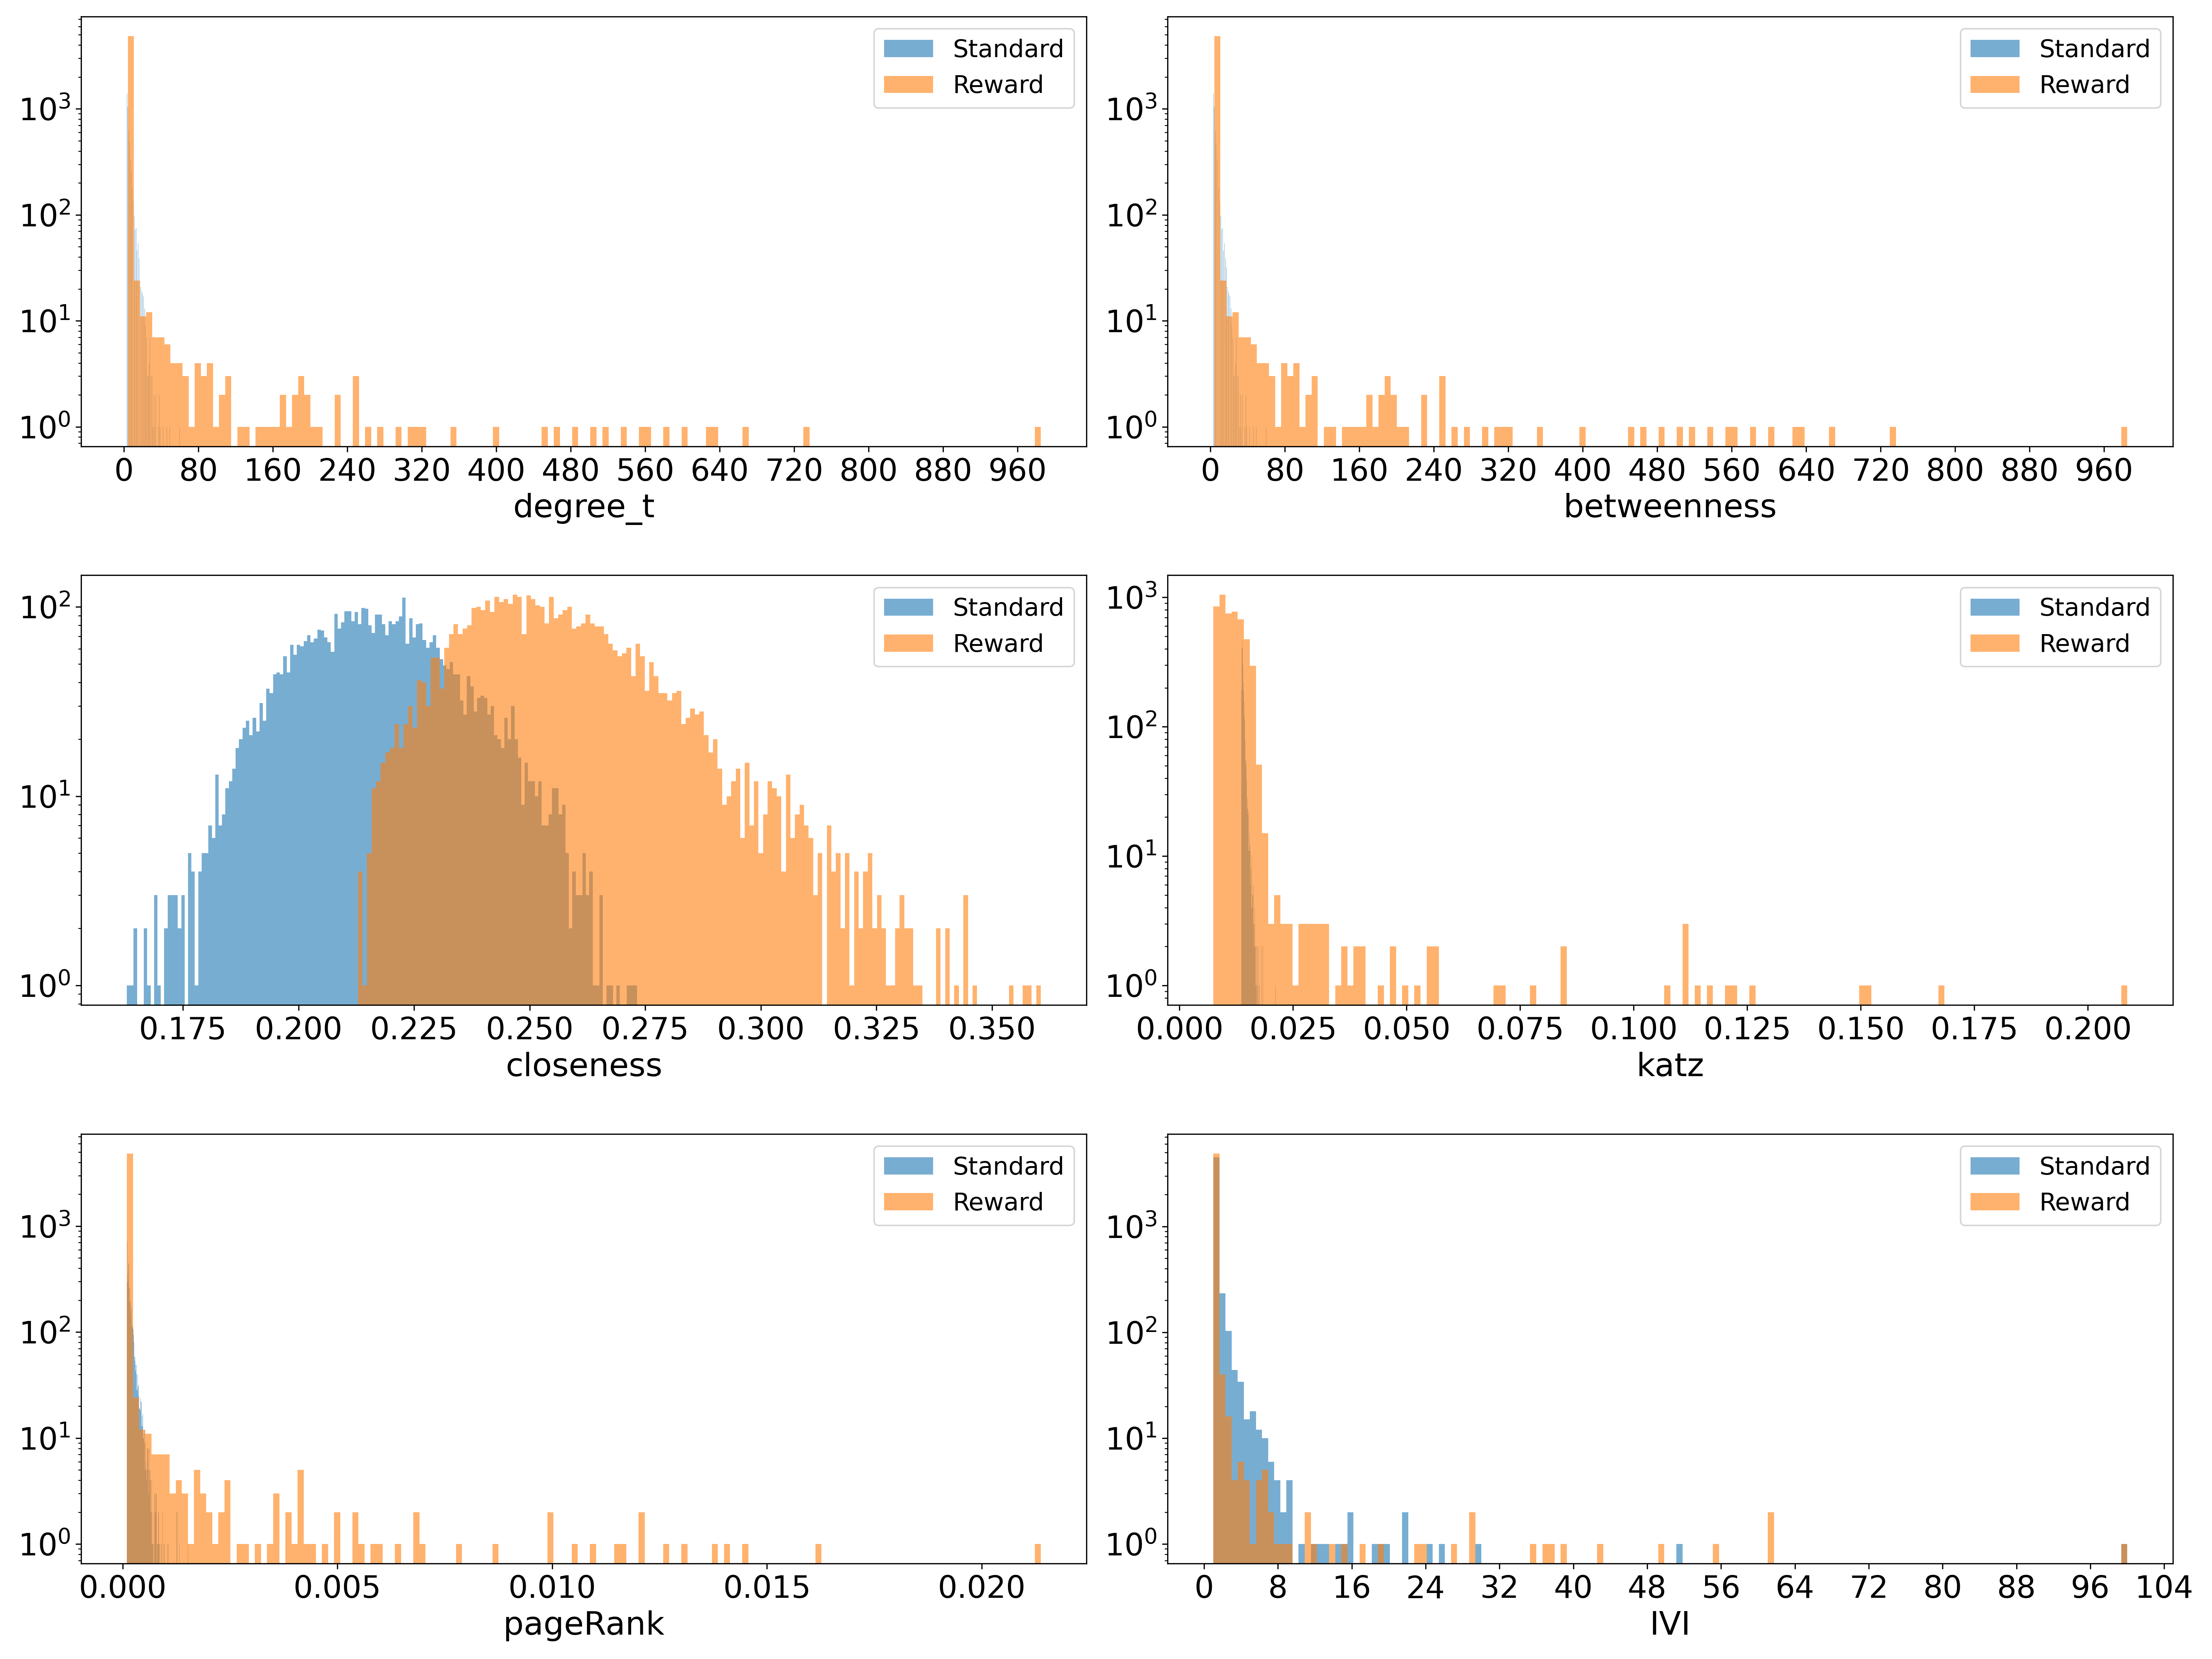
\includegraphics[width=1.0\textwidth,height=1.0\textheight,keepaspectratio]{Sections/Network_II/validation/net_metrics_Standard_Reward.png}
    \caption{Network metrics for the Standard and Sigmoid reward function. The y-axis represent the log10 of the count. }
    \label{fig:N_II:net_metric_sig_std}
\end{figure}


Through the network metrics analysis it is clear that the weight modifier have an effect on the network, but it is not evident if it is strong enough to influence the Module Connection (ModCon) scores. The 100 genes with the highest ModCon are selected which are the ones also used to stratify the MIBC. \Cref{fig:N_II:modCon_modifiers} addresses this by looking at the distribution of the mutation burden (or mutation count) from TCGA over the normalised ModCon values\footnote{The ModCon scores are normalised as the communities vary in size.}. 

For each community the 100 chosen genes are then ranked by their ModCon score which are then normalised\footnote{The ModCon Ranks are normalised in order to account for community size imbalance}. A value of 1 on the X-axis signals a high important gene while 0 the opposite. This means, that the importance increases from left to right. The comparison is done for both tumour and non-tumour generated networks for the standard (blue), Reward 1 (orange) and Reward 2 (green - Sigmoid) modifiers. 

\begin{figure}[H]
    \centering
    \begin{subfigure}{1.0\linewidth}
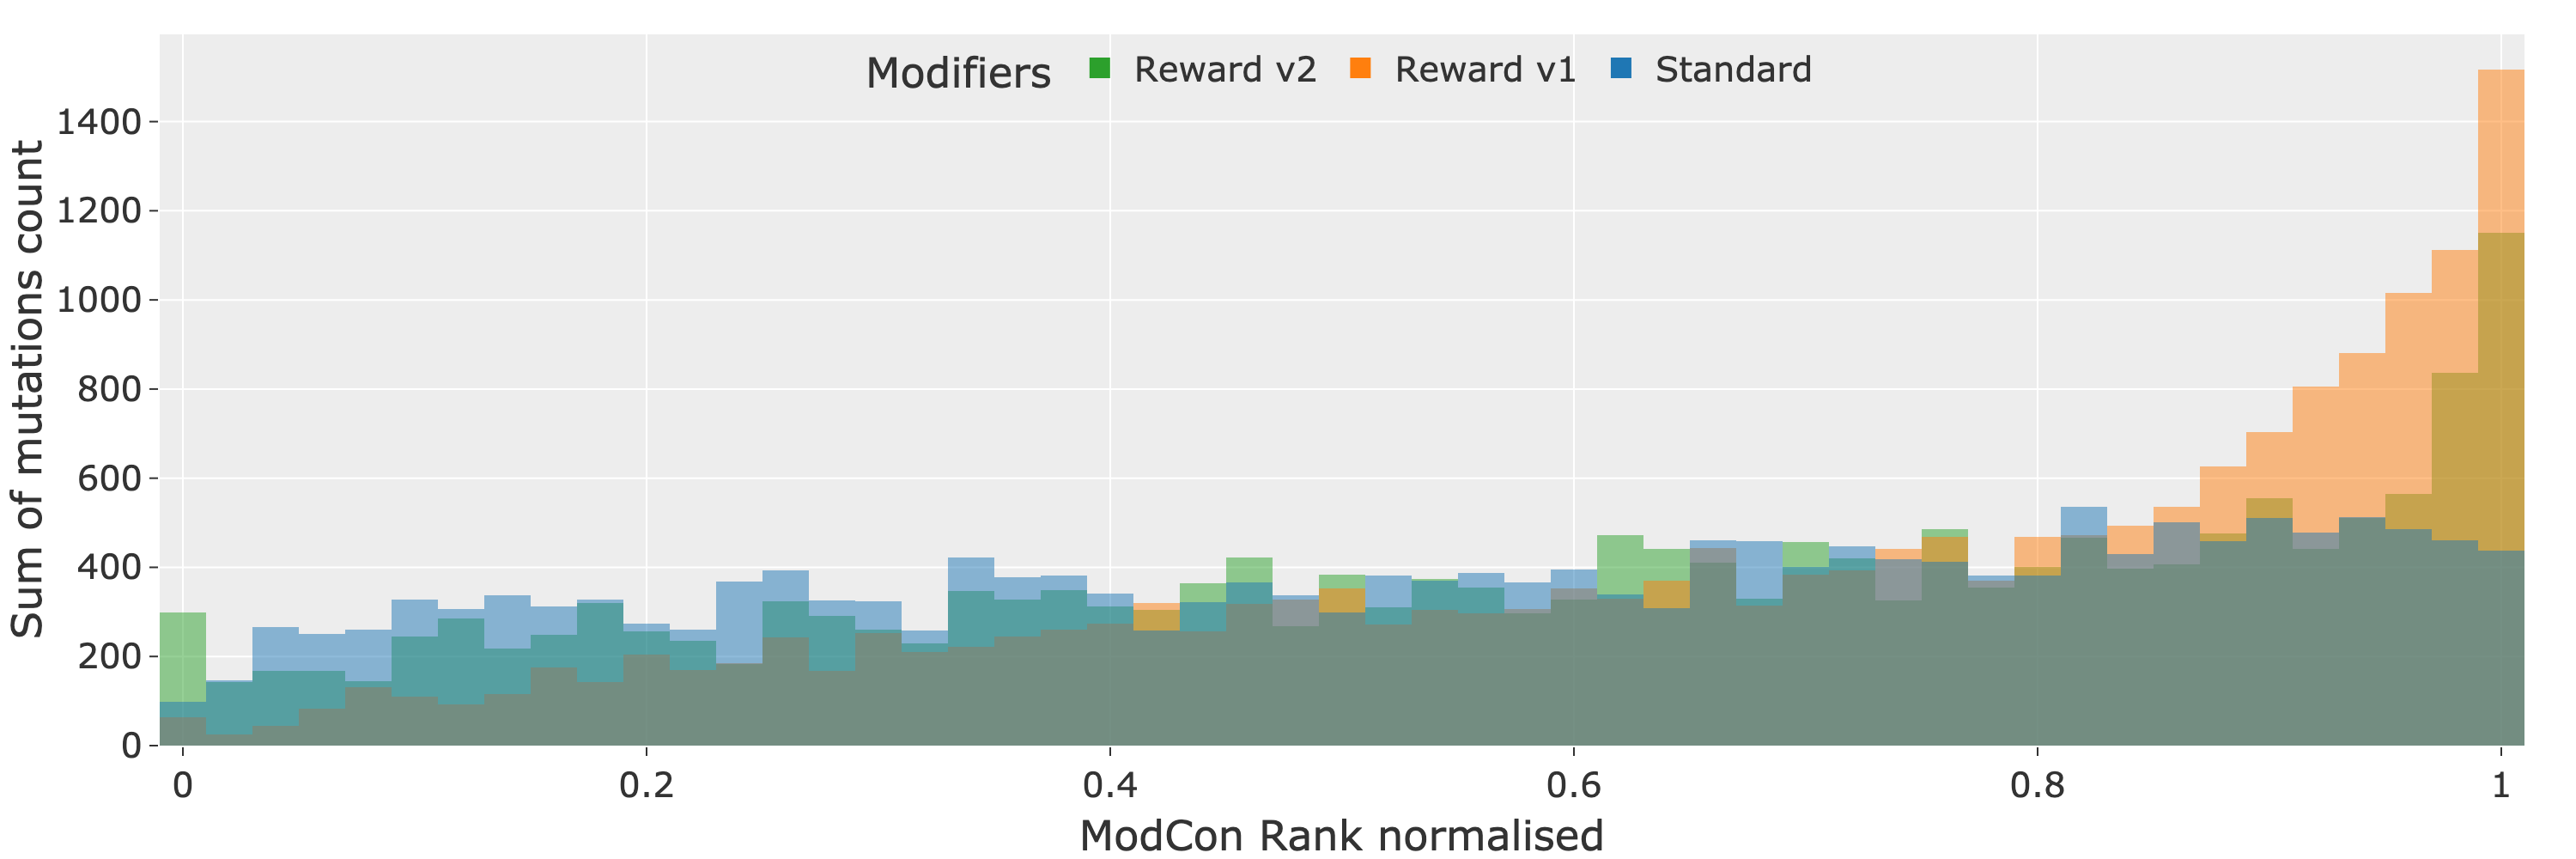
\includegraphics[width=1.0\textwidth,height=1.0\textheight,keepaspectratio]{Sections/Network_II/validation/tum_modCon_hist_2.png}
        \caption{Networks generated from the tumour dataset (TCGA)}
    \end{subfigure} %
    \centering
    \begin{subfigure}{1.0\linewidth}
        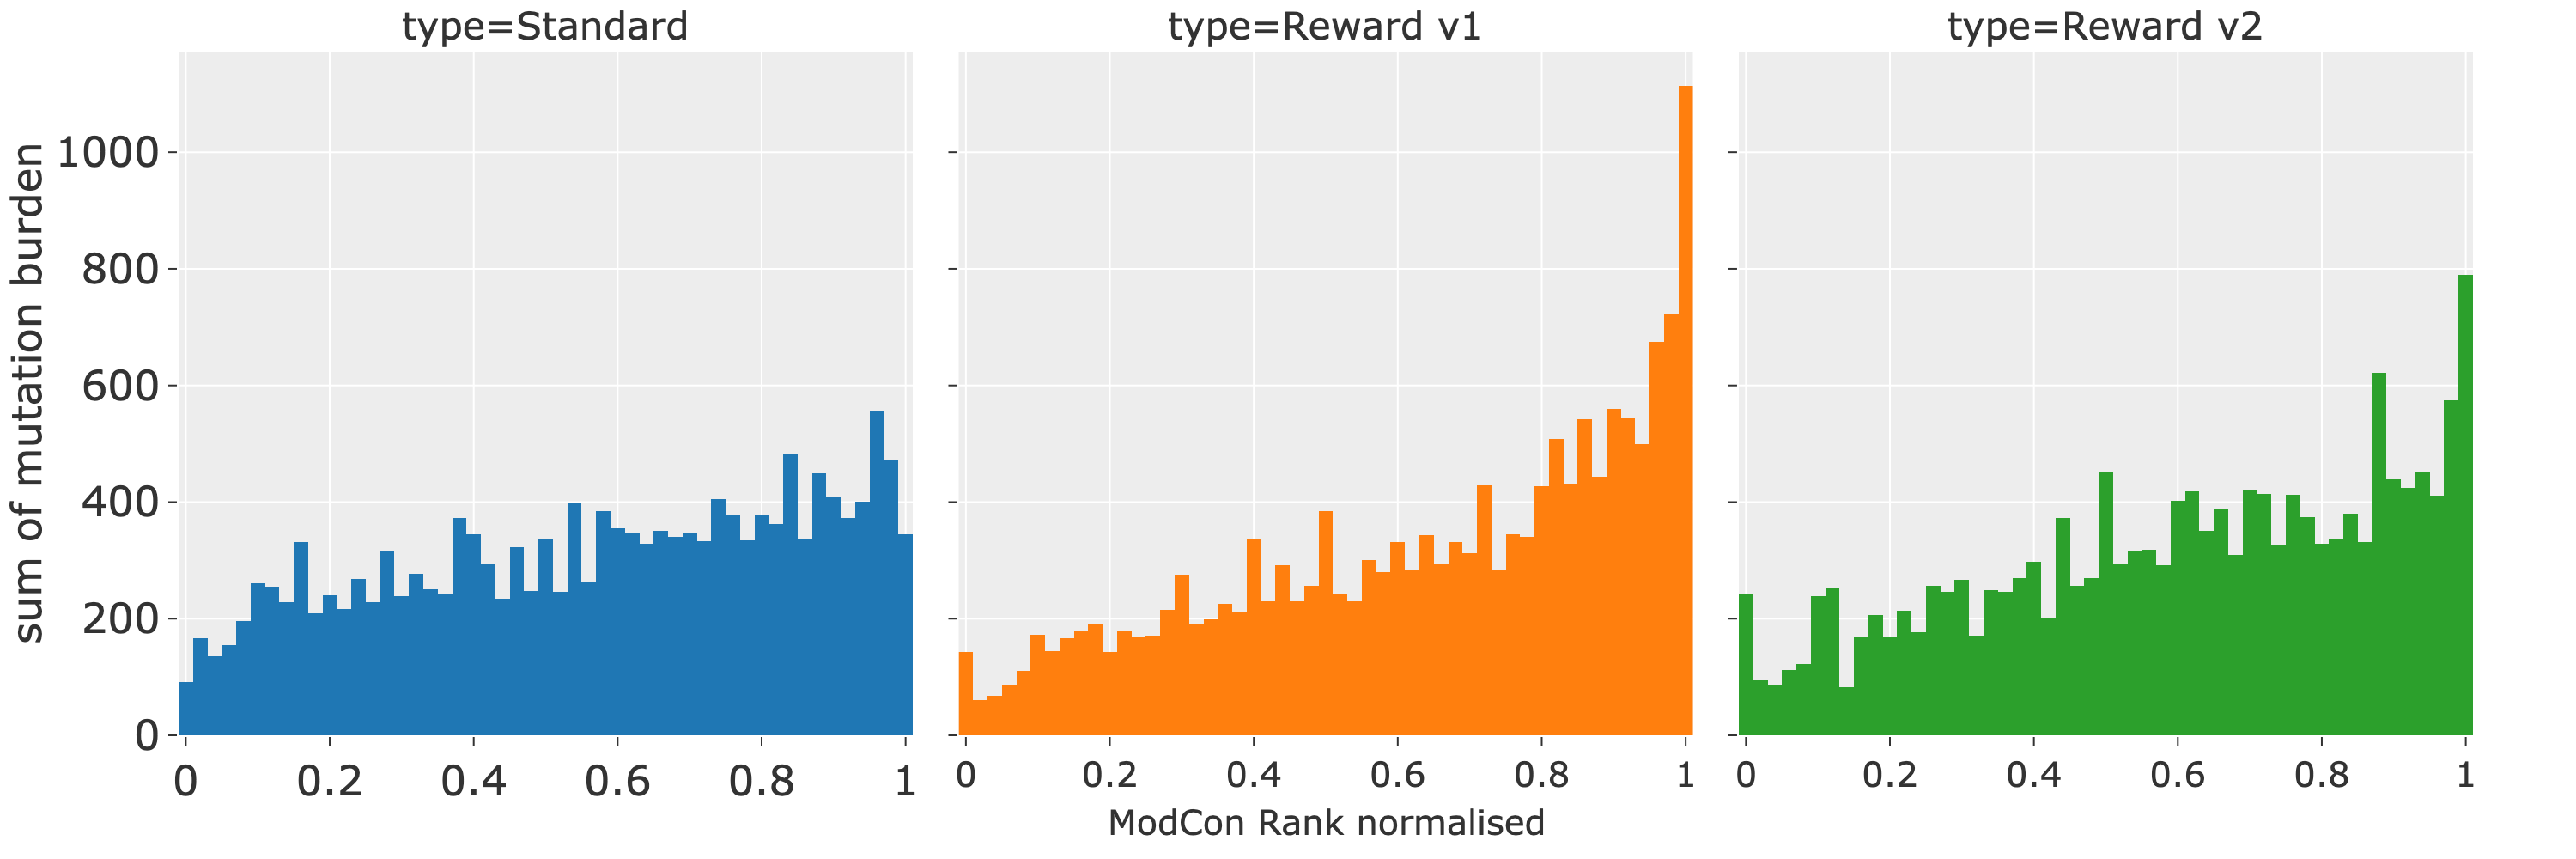
\includegraphics[width=1.0\textwidth, ,height=1.0\textheight,keepaspectratio]{Sections/Network_II/validation/non_tum_modCon_hist_2.png}
        \caption{Networks generated from the non-tumour dataset (JBU)}
    \end{subfigure}
    \centering
    \caption{The mutation burden from TCGA (Y-axis) over the ModCon Ranking (X-axis) for the three weight modifiers: standard, Reward 1 and Reward 2 (sigmoid). The relation between mutations and node's community relevance is shown for both tumour and non-tumour networks.}
    \label{fig:N_II:modCon_modifiers}
\end{figure}

% Discuss the impact of Reward v1
The two histograms in \cref{fig:N_II:modCon_modifiers} show that the sigmoid modifier (Reward v2) has the intended effect on the ModCon. In both cases, the cumulative mutation burden of the selected genes increases with the ModCon ranks. In contrast, the previous modifier (Reward v1) results in a steep increase towards the higher-ranked nodes, while at the lower ranks, only a few genes are mutated. The steep increase in the first version of the weight modifier also leads to having the most mutated genes at high ModCon across the three networks.

Overall, the two histograms in \cref{fig:N_II:modCon_modifiers} demonstrate the effects of the weight modifiers and confirm the intended behaviour of the sigmoid version. It is also worth noting the difference between the tumour and non-tumour datasets. The former has a high concentration of the mutation burden at the high ranks of the ModCon scores, indicating that gene expression reflects tumour abnormalities.


% iMEV comparison
\subsection{MEV comparisons} \label{s:N_II:mev_comp}

Towards the last stages of the network pipeline there is the MEV score which bridges the gap between the gene to sample representation. This chapter introduced a new MEV score that integrates the gene expression from both the tumour and non-tumour as explained in \cref{s:N_II:iMEV}.

To validate the change in the MEV, the non-tumour networks of $5,000$ genes, with $3$ genes per non-TF gene and $6$ for TF and hierarchical SBM was applied to determine the communities. Both standard and reward v2 networks were used for comparison. To be consistent with previous work, K-means with K=6 was used to compare the subgroups by the two MEV versions.

The results of the comparison are shown in \cref{fig:N_II:mevs_comp}, presenting the subtypes derived using the different MEVs scores, MEV\_1 (first iteration) and MEV\_2 (second iteration - integrative), in relation to previous classification. In the top comparison, where the subtypes derived from the standard networks, there is some change between the groups found using the two version of MEV scores. Nevertheless, the integrative MEV is more powerful in the reward-derived networks as seen in bottom Sankey plot. There is a subset of samples that switch from group 0 (Reward\_MEV\_1) to 3 (Reward\_MEV\_3) which has a considerable implication to the subtypes. It was observed by varying the size of $K$ that as the number of groups for K-means is increased, the difference between the two MEVs also increases. 


The comparisons validating that updating the MEV to integrate both gene expressions has an a relative low impact on the MIBC subtyping. Nevertheless, the integrative MEV (iMEV) is a better representation of the goals and aims of the project.


\begin{figure}[!htb]
    \centering
    \begin{subfigure}{1.0\linewidth}
        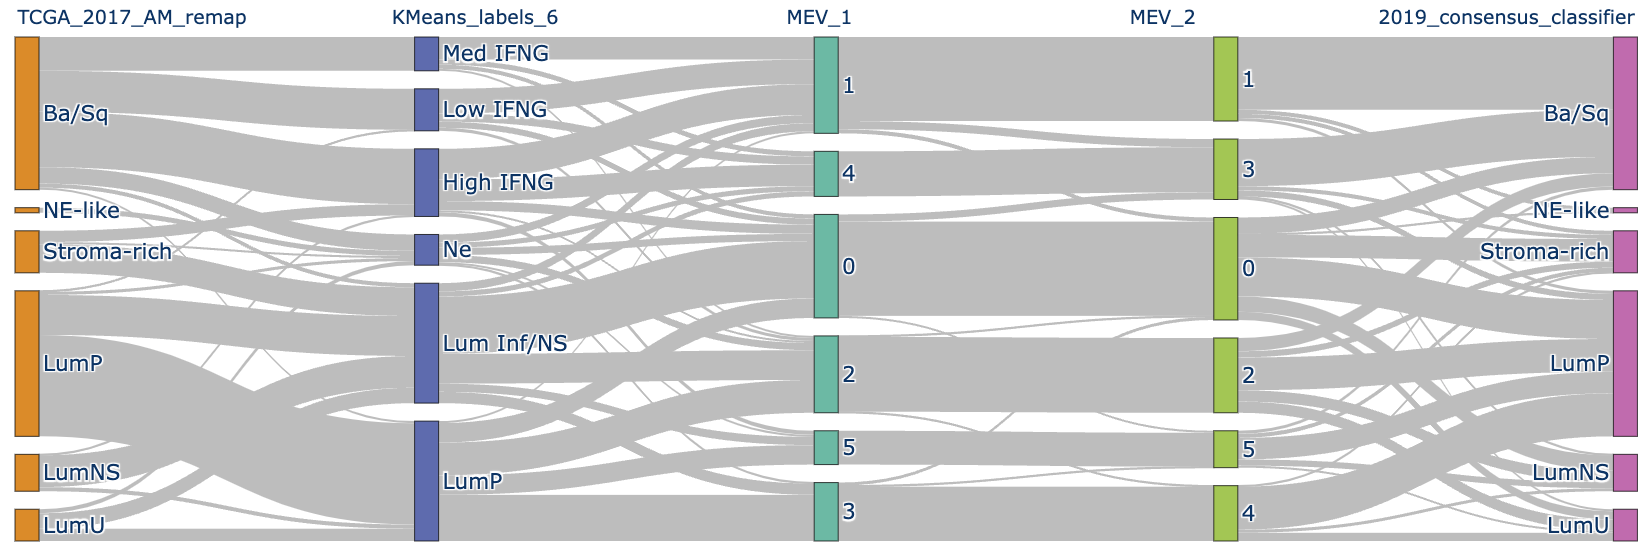
\includegraphics[width=1.0\textwidth,keepaspectratio]{Sections/Network_II/validation/mevs_comp_std.png}
        \caption{Standard networks}
    \end{subfigure} %
    \centering
    \begin{subfigure}{1.0\linewidth}
        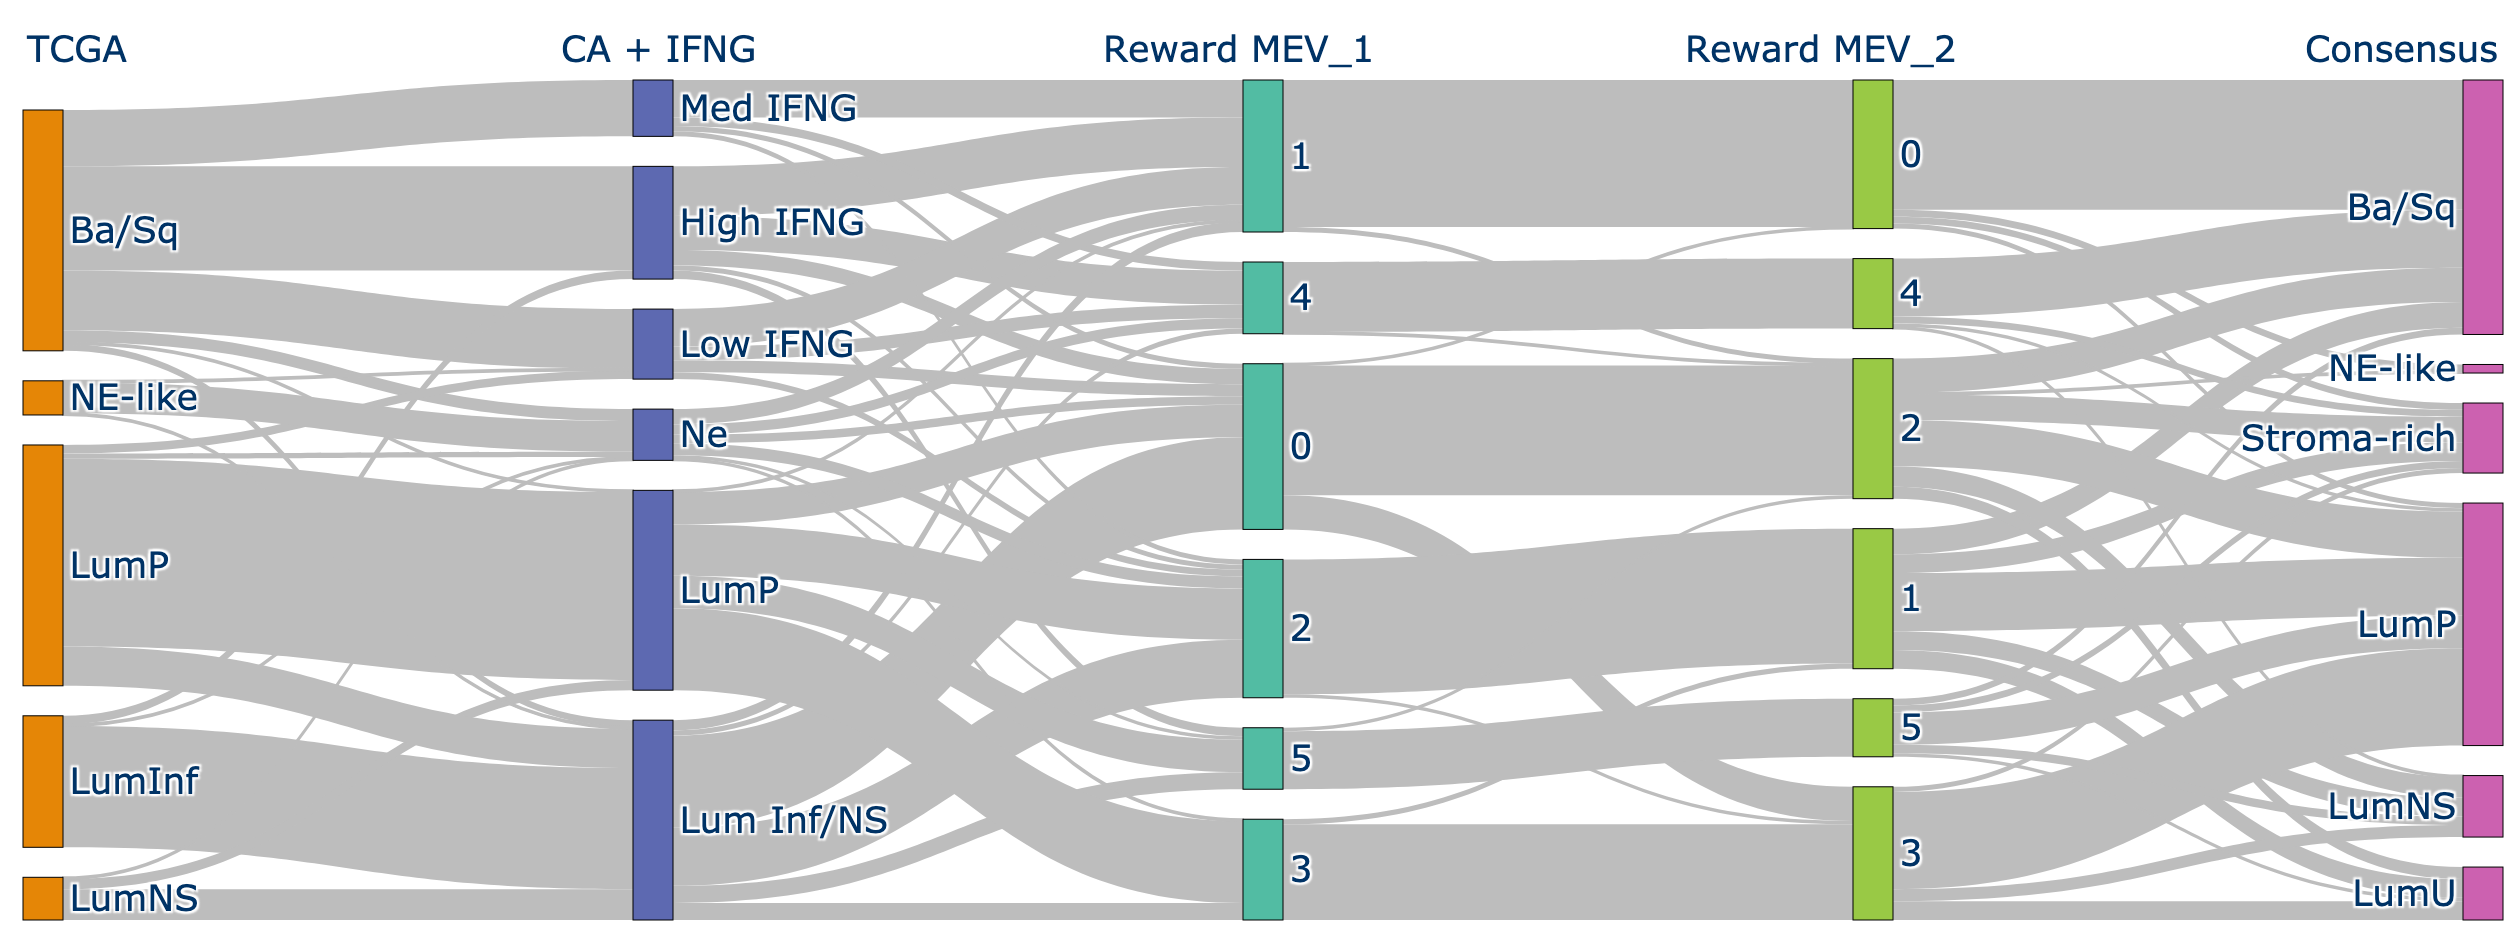
\includegraphics[width=1.0\textwidth,keepaspectratio]{Sections/Network_II/validation/mevs_comp_rwd.png}
        \caption{Reward v2 networks}
    \end{subfigure}
    \centering
    \caption{In both subfigures, sankey comparison between the TCGA classification \citet{Robertson2017-mg}, the previous MIBC stratification derived in this PhD \cref{s:cs:bio_interp}, the two version of MEVs and the consensus \citet{Kamoun2020-tj}. The difference in the plots come from comparing the standard and reward together. The subtyping based on the two MEVs are the main groups to compare as the version of MEV only considers the gene expression from the TCGA cohort while the second it integrates the non-tumour dataset as well; the other classifications are used for reference.}
    \label{fig:N_II:mevs_comp}
\end{figure}

